\subsection{Sequence Diagram}
\\\\
\begin{figure}[h]
\centering
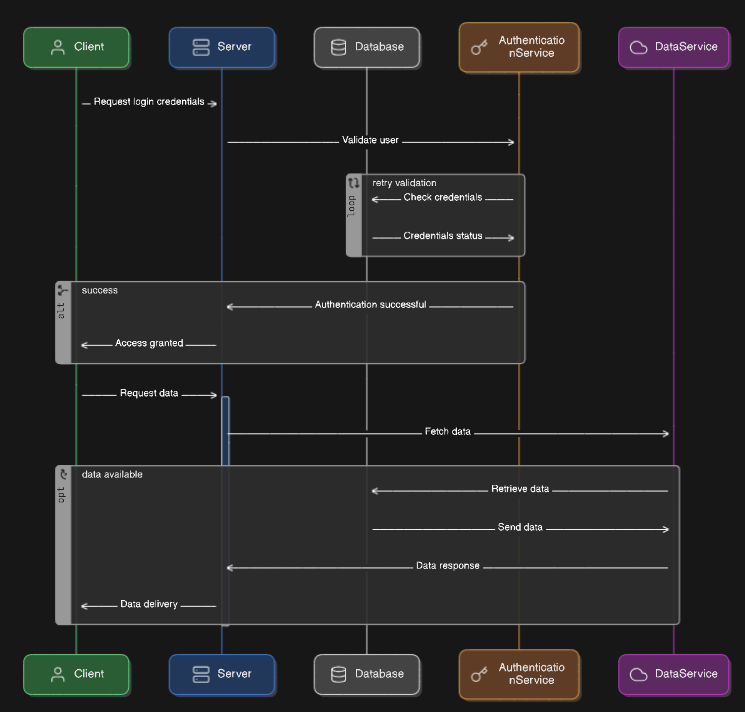
\includegraphics[width=0.8\textwidth, inner]{sections/BLL/LoginSequenceDiagram.png}
\caption{Login Sequence diagram}
\end{figure}\\
\textbf{Description:}\\ The login process begins when the client sends a request to the server with the user's credentials. The server verifies the provided username and password against stored data. If the credentials are valid, the server responds with a success message, granting the user access. This sequence diagram outlines the essential steps involved in the login process and emphasizes the importance of authentication for system security.\newpage

\begin{figure}[h]
\centering
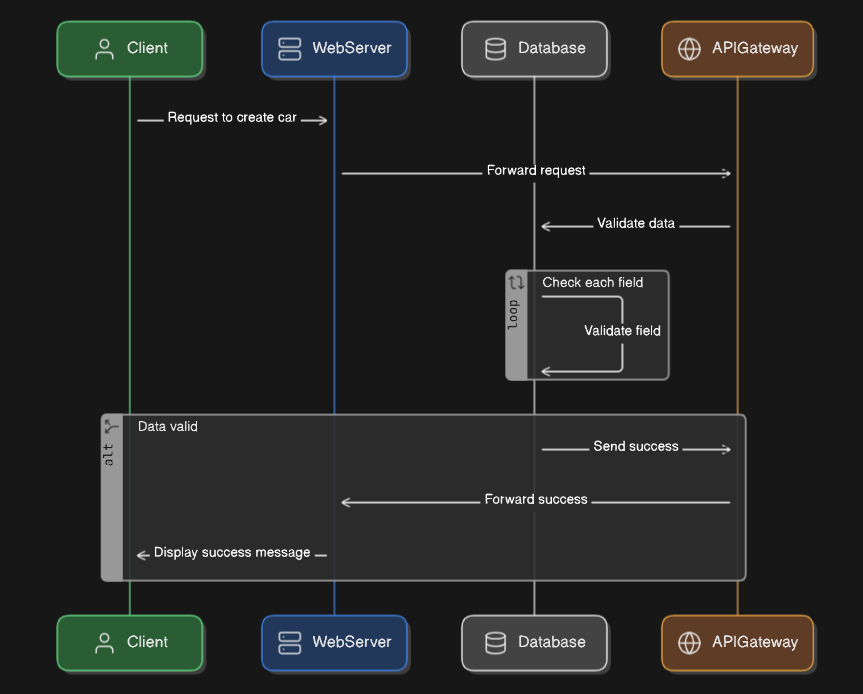
\includegraphics[width=0.8\textwidth, inner]{sections/BLL/CarSequenceDiagram.png}
\caption{Car Sequence Diagram}
\label{fig:figure2}
\end{figure}
\textbf{Description:}\\
The car sequence diagram illustrates the process flow involved in managing cars within the system. It visually depicts the interactions between various components, including clients, servlets, DAOs (Data Access Objects), resources, and databases.\\
In this sequence, the client initiates the process by sending a request to the server, often facilitated by a servlet. The servlet then communicates with the appropriate DAO to perform operations related to cars, such as creation, updating, or reservation. The DAO interacts with the database to retrieve or modify car-related data accordingly.\\
For instance, in a car reservation scenario, the sequence might show the client requesting to reserve a car. The servlet processes this request and communicates with the reservation DAO to verify car availability and update the reservation status in the database. Finally, the servlet responds to the client, indicating the success or failure of the reservation process.\\
Overall, the car sequence diagram provides a visual representation of the steps involved in managing cars within the system, aiding in understanding the process flow and interactions between different system components.\newpage
\begin{figure}[h]
\centering
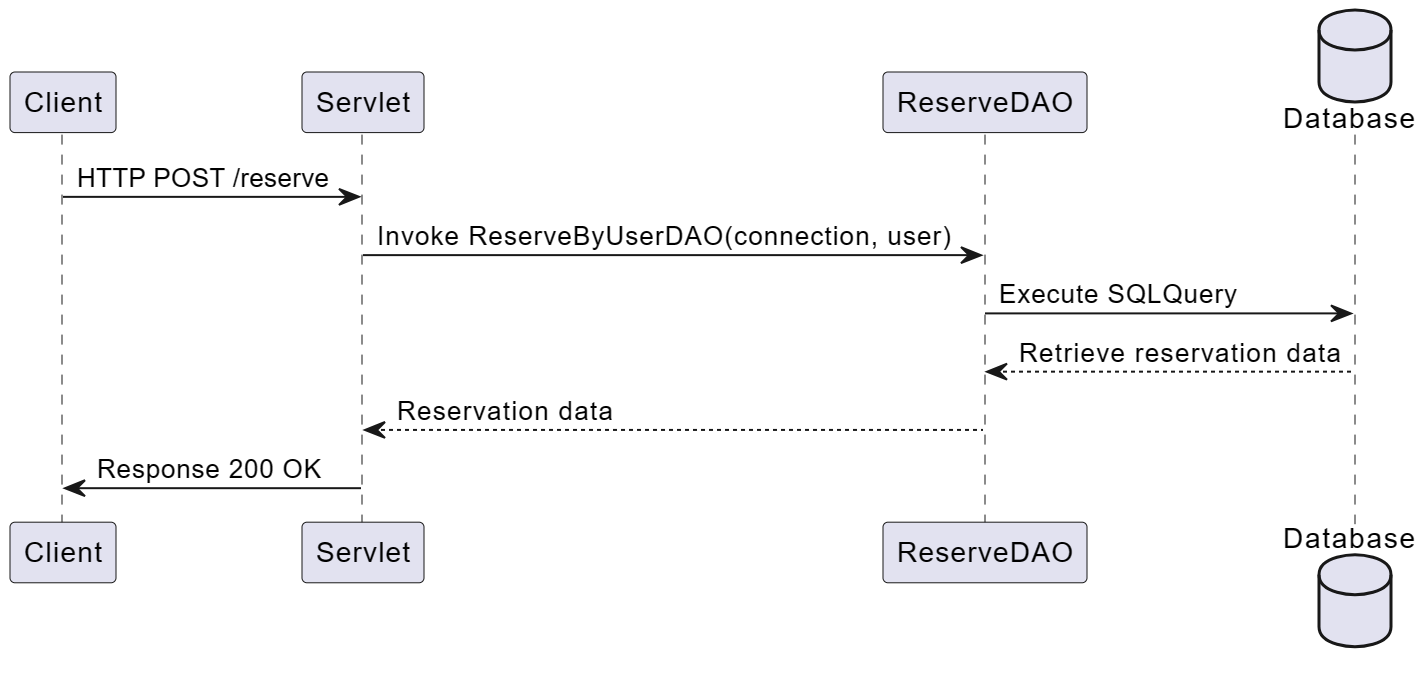
\includegraphics[width=0.9\textwidth, inner]{sections//BLL/Reserve-Sequence-diagram.png}
\caption{Reserve Sequence Diagram}
\label{fig:figure2}
\end{figure}
%describe here the sequence diagram
\textbf{Description:}\\
The car reservation sequence diagram illustrates the process of reserving a car within the system.\\
The client initiates the process by sending an HTTP POST request to the servlet, triggering a series of interactions. The servlet interacts with the ReserveDAO to access the database and retrieve reservation data for the specified user. Following this, the database processes the request, retrieves the necessary data, and returns it to the servlet. Finally, the servlet responds to the client with an HTTP status code of 200 OK, indicating a successful reservation.\\
This sequence diagram provides a clear overview of the interactions involved in the car reservation process, from client request to server response.\newpage